\documentclass{beamer}
\renewcommand\thesection{\arabic{section}}
\newcommand{\myfont}{\rmfamily\normalsize\upshape\mdseries}
\newcommand{\degree}{^\circ}
\title{\sffamily Review III(Slides 177 - 225)}
\subtitle{\textbf{Poset \& Cardinality}\\}
\institute[UM-SJTU JI]{University of Michigan-Shanghai Jiao Tong University Joint Institute}
\author{HamHam}
\usepackage{graphicx}
\usepackage{picinpar}
\usepackage{indentfirst}
\usepackage{chemformula}
\usepackage{geometry}
\usepackage{subfigure}
\usepackage{appendix}
\usepackage{amsfonts,amsmath,amssymb}
\usepackage{bm,bbm}
\usepackage{enumerate}
\usepackage{float}
\usepackage{geometry}
\usepackage{latexsym}
\usepackage{listings}
\usepackage{multicol,multirow,multido}
\usepackage{tabularx}
\usepackage{ulem}
\usepackage{tikz}
\usepackage{color,xcolor}
\usepackage{cite}
\usepackage{setspace}
\usepackage{hyperref}
\usepackage{textpos}
\usepackage{booktabs}
\usepackage{diagbox}
\usepackage{pgfplots}
\usepackage{listings}
\usepackage{graphics}
\usepackage{upgreek}
%定义绘制椭圆的命令,带有四个参数
%第一个参数:椭圆位置的横坐标
%第二、三参数:椭圆x位置的半径、y位置的半径
%第四个参数:填充的透明度
\def\drawell#1#2#3#4{
	\draw[draw=black,fill=gray,fill opacity=#4,line width=3pt] 
	(#1,0) circle [x radius=#2, y radius=#3];}

%%%%%%%%%%%%%%%%%%%%%%%%%%%%%%%%%%%%%%%%%%%%%%%%%%%%%%%%%%%%%%%%%%%%%%%%%%%%%
\iffalse 
Copyright 2021 by Leyang Zhang, Yinchen Ni, Yuxiang Chen, Yue Huang

You should not spread this file without the permission from every one of 
    Leyang Zhang, Yinchen Ni and Yuxiang Chen 
\fi
%%%%%%%%%%%%%%%%%%%%%%%%%%%%%%%%%%%%%%%%%%%%%%%%%%%%%%%%%%%%%%%%%%%%%%%%%%%%%

\ProvidesPackage{JI_MathCourse_Notations}[2021/12/19]

\RequirePackage{amsmath}
\RequirePackage{amsthm}
\RequirePackage{amssymb}
\RequirePackage{bm}
\RequirePackage{bbm}
\RequirePackage{color}


%Typesetting

%colors 
\newcommand{\blue}[1]{\textcolor{blue}{#1}}                         %blue
\newcommand{\cha}[1]{\textcolor[rgb]{0.95,0.75,0.9}{#1}}            %cha-type color 
\newcommand{\gray}[1]{\textcolor{gray}{#1}}                         %grey
\newcommand{\pink}[1]{\textcolor{pink}{#1}}                         %pink
\newcommand{\red}[1]{\textcolor[rgb]{0.75,0,0}{#1}}                 %red
\newcommand{\yellow}[1]{\textcolor{orange}{#1}}                     %yellow
\newcommand{\green}[1]{\textcolor[rgb]{0,0.6,0.2}{#1}}

%declarations of Math lines, turn off code checker before using them
\newcommand{\beq}{\begin{equation}}
\newcommand{\beqa}{\begin{equation}\begin{aligned}}
\newcommand{\beqNo}{\begin{equation*}}
\newcommand{\beqaNo}{\begin{equation*}\begin{aligned}}
\newcommand{\eeq}{\end{equation}}
\newcommand{\eeqa}{\end{aligned}\end{equation}}
\newcommand{\eeqNo}{\end{equation*}}
\newcommand{\eeqaNo}{\end{aligned}\end{equation*}}

%space 
\newcommand{\hh}{\hspace{1em}}
\newcommand{\hs}[1]{\hspace{#1}}
\newcommand{\vs}[1]{\vspace{#1}}
\newcommand{\vv}{\vspace{1em}}


%-------------------------------------------------------------------


%Letter-like Notations 

%A - Z notations 
\newcommand{\bA}{\mathbb{A}}    \newcommand{\calA}{\mathcal{A}}     \newcommand{\fA}{\mathfrak{A}}
\newcommand{\bB}{\mathbb{B}}    \newcommand{\calB}{\mathcal{B}}     \newcommand{\fB}{\mathfrak{B}} 
\newcommand{\bC}{\mathbb{C}}    \newcommand{\calC}{\mathcal{C}}     \newcommand{\fC}{\mathfrak{C}} 
\newcommand{\bD}{\mathbb{D}}    \newcommand{\calD}{\mathcal{D}}     \newcommand{\fD}{\mathfrak{D}} 
\newcommand{\bE}{\mathbb{E}}    \newcommand{\calE}{\mathcal{E}}     \newcommand{\fE}{\mathfrak{E}} 
\newcommand{\bF}{\mathbb{F}}    \newcommand{\calF}{\mathcal{F}}     \newcommand{\fF}{\mathfrak{F}} 
\newcommand{\bG}{\mathbb{G}}    \newcommand{\calG}{\mathcal{G}}     \newcommand{\fG}{\mathfrak{G}} 
\newcommand{\bH}{\mathbb{H}}    \newcommand{\calH}{\mathcal{H}}     \newcommand{\fH}{\mathfrak{H}} 
\newcommand{\bI}{\mathbb{I}}    \newcommand{\calI}{\mathcal{I}}     \newcommand{\fI}{\mathfrak{I}} 
\newcommand{\bJ}{\mathbb{J}}    \newcommand{\calJ}{\mathcal{J}}     \newcommand{\fJ}{\mathfrak{J}} 
\newcommand{\bK}{\mathbb{K}}    \newcommand{\calK}{\mathcal{K}}     \newcommand{\fK}{\mathfrak{K}}  
\newcommand{\bL}{\mathbb{L}}    \newcommand{\calL}{\mathcal{L}}     \newcommand{\fL}{\mathfrak{L}} 
\newcommand{\bM}{\mathbb{M}}    \newcommand{\calM}{\mathcal{M}}     \newcommand{\fM}{\mathfrak{M}} 
\newcommand{\bN}{\mathbb{N}}    \newcommand{\calN}{\mathcal{N}}     \newcommand{\fN}{\mathfrak{N}}  
\newcommand{\bO}{\mathbb{O}}    \newcommand{\calO}{\mathcal{O}}     \newcommand{\fO}{\mathfrak{O}} 
\newcommand{\bP}{\mathbb{P}}    \newcommand{\calP}{\mathcal{P}}     \newcommand{\fP}{\mathfrak{P}} 
\newcommand{\bQ}{\mathbb{Q}}    \newcommand{\calQ}{\mathcal{Q}}     \newcommand{\fQ}{\mathfrak{Q}} 
\newcommand{\bR}{\mathbb{R}}    \newcommand{\calR}{\mathcal{R}}     \newcommand{\fR}{\mathfrak{R}} 
\newcommand{\bS}{\mathbb{S}}    \newcommand{\calS}{\mathcal{S}}     \newcommand{\fS}{\mathfrak{S}}     
\newcommand{\bT}{\mathbb{T}}    \newcommand{\calT}{\mathcal{T}}     \newcommand{\fT}{\mathfrak{T}} 
\newcommand{\bU}{\mathbb{U}}    \newcommand{\calU}{\mathcal{U}}     \newcommand{\fU}{\mathfrak{U}} 
\newcommand{\bV}{\mathbb{V}}    \newcommand{\calV}{\mathcal{V}}     \newcommand{\fV}{\mathfrak{V}} 
\newcommand{\bW}{\mathbb{W}}    \newcommand{\calW}{\mathcal{W}}     \newcommand{\fW}{\mathfrak{W}} 
\newcommand{\bX}{\mathbb{X}}    \newcommand{\calX}{\mathcal{X}}     \newcommand{\fX}{\mathfrak{X}} 
\newcommand{\bY}{\mathbb{Y}}    \newcommand{\calY}{\mathcal{Y}}     \newcommand{\fY}{\mathfrak{Y}} 
\newcommand{\bZ}{\mathbb{Z}}    \newcommand{\calZ}{\mathcal{Z}}     \newcommand{\fZ}{\mathfrak{Z}} 

%Math-specific notations 

\newcommand{\ep}{\epsilon}                                          %epsilon
\newcommand{\vep}{\varepsilon}                                      %variable epsilon


%-------------------------------------------------------------------


%Common Operations 

%sets 
\renewcommand{\Cap}{\bigcap}                                        %A intersect with B 
\newcommand{\card}{\text{card }}                                    %cardinality of a set
\renewcommand{\Cup}{\bigcup}                                        %A union with B 
\newcommand{\cut}{\backslash}                                       %A \ B 
\newcommand{\es}{\approx}                                           %equinumerosity between two sets 
\newcommand{\nes}{\not\approx}                                      %not Equinumerosity 
\newcommand{\siq}{\subseteq}                                        %A is contained in B 
\newcommand{\soq}{\supseteq}                                        %A is out of range of B 
\newcommand{\symd}{\Delta}                                          %symmetric difference 

%functions and function-related operations 
\newcommand{\ceil}[1]{\lceil {#1} \rceil}                           %smallest integer no less than #1 
\newcommand{\dist}[2]{\text{dist}\left ({#1},{#2} \right )}         %Distance function 
\newcommand{\floor}[1]{\lfloor {#1} \rfloor}                        %largest integer no greater than #1 
\newcommand{\inv}[1]{{#1}^{-1}}                                     %the inverse of a function, a number or a group element
\renewcommand{\mod}[1]{\,(\text{mod } {#1})}                        %modular of an integer #1 
\newcommand{\ran}{\text{ran }}                                      %the range of a function
\newcommand{\inflim}[1]{\varliminf_{#1}}                            %limit infimum of sequence or set
\newcommand{\limc}[2]{\lim_{#1 \to #2}}                             %limit 
\newcommand{\suplim}[1]{\varlimsup_{#1}}                            %limit supremum of sequence or set

%Others
\newcommand{\larrow}{\leftarrow}                                    %single left arrow, implies
\newcommand{\rarrow}{\rightarrow}                                   %single right arrow, implies 
\newcommand{\Larrow}{\Leftarrow}                                    %double left arrow, implies 
\newcommand{\Rarrow}{\Rightarrow}                                   %double right arrow, implies 
\newcommand{\lrarrow}{\leftrightarrow}                              %single left-right arrow 
\newcommand{\LRarrow}{\Leftrightarrow}                              %double left-right arrow, shorter than \iff 
\newcommand{\lowBrace}[2]{\underset{#1}{\underbrace{#2}}}           %under-brace with notes 
\renewcommand{\(}{\left (}                                          %left-half bracket, turn off code checker before using it 
\renewcommand{\)}{\right )}                                         %right-half bracket, turn off code checker before using it 
\newcommand{\<}{\langle}                                            %left-half angular bracket 
\renewcommand{\>}{\rangle}                                          %right-half angular bracket


%-------------------------------------------------------------------


%Patches  

%Analysis and Calculus 
\newcommand{\df}[2]{\frac{d{#1}}{d{#2}}}                            %one-variable differential operator
%\newcommand{\indf}[2]{\dfrac{d{#1}}{d{#2}}}                         %differential operator for in-line math mode
\newcommand{\im}{\text{Im }}                                        %taking the imaginary part of a number or a function 
\newcommand{\inrPdct}[2]{\left \langle{#1},{#2}\right \rangle}      %inner product 
\newcommand{\nDf}[2]{{#1}^{({#2})}}                                 %n-th derivative of some function 
\newcommand{\norm}[1]{\left \|#1\right \|}                                       %norm 
\newcommand{\parf}[2]{\frac{\partial{#1}}{\partial{#2}}}            %partial derivative of a function 
\newcommand{\parfwide}[2]{\partial{#1} / \partial{#2}}              %partial derivative of a function, wide form 
\newcommand{\re}{\text{Re }}                                        %taking the real part of a number or a function 

%Combinatorics 
\newcommand{\al}{{\aleph}_{0}}                                      %Aleph zero 
\newcommand{\all}{{\aleph}_{1}}                                     %Aleph one
\newcommand{\dbinomial}[2]{\begin{pmatrix}\!\!
                           \begin{pmatrix}{#1}\\{#2} 
                           \end{pmatrix}
                           \!\!\!
                           \end{pmatrix}}                           %double binomial 
\newcommand{\kpermu}[2]{{#1}^\text{\underline{#2}}}                 %k-permutation 
\newcommand{\logs}{\log^{*}}                                        %Iterated Logarithm 
\newcommand{\stirling}[2]{\left \{\begin{aligned} 
                                    {#1} \\ {#2} 
                                  \end{aligned} 
                          \right \}}                                %Stirling numbers of second kind 

%Graph Theory 
\newcommand{\comp}[1]{\text{comp} \left({#1}\right)}                %Component of graph 
\newcommand{\conj}{\overline}                                       %Complement graph of a given graph

%intersection of a collection of sets indexed by I 
\newcommand{\AI}{\cap_{i \in I} A_i} 
\newcommand{\BI}{\cap_{i \in I} B_i} 
\newcommand{\CI}{\cap_{i \in I} C_i} 
\newcommand{\DI}{\cap_{i \in I} D_i} 
\newcommand{\EI}{\cap_{i \in I} E_i} 
\newcommand{\FI}{\cap_{i \in I} F_i} 
\newcommand{\GI}{\cap_{i \in I} G_i} 
\newcommand{\HI}{\cap_{i \in I} H_i} 
\newcommand{\II}{\cap_{i \in I} I_i} 
\newcommand{\JI}{\cap_{i \in I} J_i} 
\newcommand{\KI}{\cap_{i \in I} K_i} 
\newcommand{\LI}{\cap_{i \in I} L_i} 
\newcommand{\MI}{\cap_{i \in I} M_i} 
\newcommand{\NI}{\cap_{i \in I} N_i} 
\newcommand{\OI}{\cap_{i \in I} O_i} 
\newcommand{\PI}{\cap_{i \in I} P_i} 
\newcommand{\QI}{\cap_{i \in I} Q_i} 
\newcommand{\RI}{\cap_{i \in I} R_i} 
%\renewcommand{\SI}{\cap_{i \in I} S_i}                             %\SI already defined, delete '%' if you want to renew it 
\newcommand{\TI}{\cap_{i \in I} T_i} 
\newcommand{\UI}{\cap_{i \in I} U_i} 
\newcommand{\VI}{\cap_{i \in I} V_i} 
\newcommand{\WI}{\cap_{i \in I} W_i} 
\newcommand{\XI}{\cap_{i \in I} X_i} 
\newcommand{\YI}{\cap_{i \in I} Y_i}
\newcommand{\ZI}{\cap_{i \in I} Z_i}                                

%limit as "letter" tends to infinity 
\newcommand{\limftya}{\lim_{a \to \infty}}                          
\newcommand{\limftyb}{\lim_{b \to \infty}} 
\newcommand{\limftyc}{\lim_{c \to \infty}} 
\newcommand{\limftyd}{\lim_{d \to \infty}} 
\newcommand{\limftye}{\lim_{e \to \infty}} 
\newcommand{\limftyf}{\lim_{f \to \infty}} 
\newcommand{\limftyg}{\lim_{g \to \infty}} 
\newcommand{\limftyh}{\lim_{h \to \infty}}
\newcommand{\limftyi}{\lim_{i \to \infty}}                          
\newcommand{\limftyj}{\lim_{j \to \infty}}                          
\newcommand{\limftyk}{\lim_{k \to \infty}}
\newcommand{\limftyl}{\lim_{l \to \infty}}
\newcommand{\limftym}{\lim_{m \to \infty}}
\newcommand{\limftyn}{\lim_{n \to \infty}}                          
\newcommand{\limftyo}{\lim_{o \to \infty}} 
\newcommand{\limftyp}{\lim_{p \to \infty}} 
\newcommand{\limftyq}{\lim_{q \to \infty}}
\newcommand{\limftyr}{\lim_{r \to \infty}}
\newcommand{\limftys}{\lim_{s \to \infty}}
\newcommand{\limftyt}{\lim_{t \to \infty}}
\newcommand{\limftyu}{\lim_{u \to \infty}}
\newcommand{\limftyv}{\lim_{v \to \infty}}
\newcommand{\limftyw}{\lim_{w \to \infty}} 
\newcommand{\limftyx}{\lim_{x \to \infty}}                          
\newcommand{\limftyy}{\lim_{y \to \infty}}                          
\newcommand{\limftyz}{\lim_{z \to \infty}} 

%matrices 
\newcommand{\colTwo}[2]{\begin{pmatrix}
                        #1 \\ #2 
                        \end{pmatrix}}                              %length-two column vector 
\newcommand{\colThree}[3]{\begin{pmatrix}
                        #1 \\ #2 \\ #3
                        \end{pmatrix}}                              %length-three column vector 
\newcommand{\colFour}[4]{\begin{pmatrix}
                        #1 \\ #2 \\ #3 \\ #4 
                        \end{pmatrix}}                              %length-four column vector 
\newcommand{\colFive}[5]{\begin{pmatrix}
                        #1 \\ #2 \\ #3 \\ #4 \\ #5
                        \end{pmatrix}}                              %length-five column vector 
\newcommand{\diagTwo}[2]{\begin{pmatrix} 
                         #1 &\, \\ 
                         \, &#2 \\ 
                         \end{pmatrix}}                             %two-by-two diagonal matrix 
\newcommand{\diagThree}[3]{\begin{pmatrix} 
                           #1 &\, &\, \\ 
                           \, &#2 &\, \\ 
                           \, &\, &#3 \\ 
                           \end{pmatrix}}                           %three-by-three diagonal matrix 
\newcommand{\diagFour}[4]{\begin{pmatrix} 
                           #1 &\, &\, &\, \\ 
                           \, &#2 &\, &\, \\ 
                           \, &\, &#3 &\, \\ 
                           \, &\, &\, &#4 \\ 
                           \end{pmatrix}}                           %four-by-four diagonal matrix }
\newcommand{\maTwo}[4]{\begin{pmatrix} 
                        #1 &#2 \\  
                        #3 &#4 \\ 
                       \end{pmatrix}}                               %two-by-two matrix
\newcommand{\maTwoThree}[6]{\begin{pmatrix} 
                            #1 &#2 &#3 \\ 
                            #4 &#5 &#6 \\ 
                            \end{pmatrix}}                          %two-by-three matrix
\newcommand{\maThreeTwo}[6]{\begin{pmatrix}
                            #1 &#2 \\ 
                            #3 &#4 \\ 
                            #5 &#6 \\ 
                            \end{pmatrix}}                          %three by two matrix 
\newcommand{\maThree}[9]{\begin{pmatrix}
                         #1 &#2 &#3 \\ 
                         #4 &#5 &#6 \\ 
                         #7 &#8 &#9 \\ 
                         \end{pmatrix}}                             %three by three matrix

%determinants 
\newcommand{\deTwo}[4]{\det \begin{pmatrix}
                            #1 &#2 \\ 
                            #3 &#4 \\ 
                            \end{pmatrix}}                          %determinant of two by two matrix 
\newcommand{\deThree}[9]{\det \begin{pmatrix}
                              #1 &#2 &#3 \\ 
                              #4 &#5 &#6 \\ 
                              #7 &#8 &#9 \\ 
                              \end{pmatrix}}                        %determinant of three by three matrix 

%span 
\renewcommand{\span}{\text{span }}                                  %the linear span of a set
\newcommand{\spans}[1]{\text{span} \{#1\}}                          %the linear span of elements 

%Topology
\newcommand{\hBall}[2]{B_{#1}\left(#2\right)}                   %B_#1 (#2): open ball centered at #2 with radius #1 
\usetheme[dove]{Boadilla}
\usecolortheme{dolphin}
%\pgfdeclaremask{figmask}{or_circuit.jpg}
%\pgfdeclareimage[mask=figmask,width=0.6\textwidth]{or_circuit}{or_circuit_1.png}
\useoutertheme{miniframes}
\begin{document}
    \usebackgroundtemplate{\tikz\node[opacity=0.25]{
    
\includegraphics[width=\paperwidth,
    height=\paperheight]{hamster.jpg}
    };}
\begin{titlepage}
    \begin{center}
        VE203 - Discrete Mathmatics 
    \end{center}
\end{titlepage}
\myfont
\section{Partial Order}
\begin{frame}
    \frametitle{Definition}
    \parbox{\textwidth}{
		\par A (binary) relation $R$ on $A$, \textit{i.e.,} $R \subset A \times A$, is
		\begin{itemize}
			\item[-] \textbf{ref\mbox{l}exive} if $aRa \Rightarrow \top$.
			\item[-] \textbf{symmetric} if $aRb \Leftrightarrow bRa$.
			\item[-] \textbf{transitive} if $aRb \wedge bRc \Rightarrow aRc$.
			\item[-] \textbf{anti-symmetric} if $aRb \wedge bRa \Rightarrow a = b$.
			\item[-] asymmetric if $aRb \wedge bRa \Rightarrow \perp$.
			\item[-] total if $aRb \vee bRa \Rightarrow \top$.
		\end{itemize}
		\par \phantom{ji}
		\par \textbf{(Non-strict) Partial order}: reflexive, antisymmetric, and transitive.
		\par \textbf{Equivalence relation}: reflexive, symmetric, and transitive.
        \par \textbf{Total order:} Partial order + total.
    }
\end{frame}
\begin{frame}
    \frametitle{Partial Order}
    \fbox{
	\parbox{0.95\textwidth}{
    \hh The term partial order typically refers to a \textbf{non-strict} 
    partial order relation.
	\par \phantom{ji}\\
	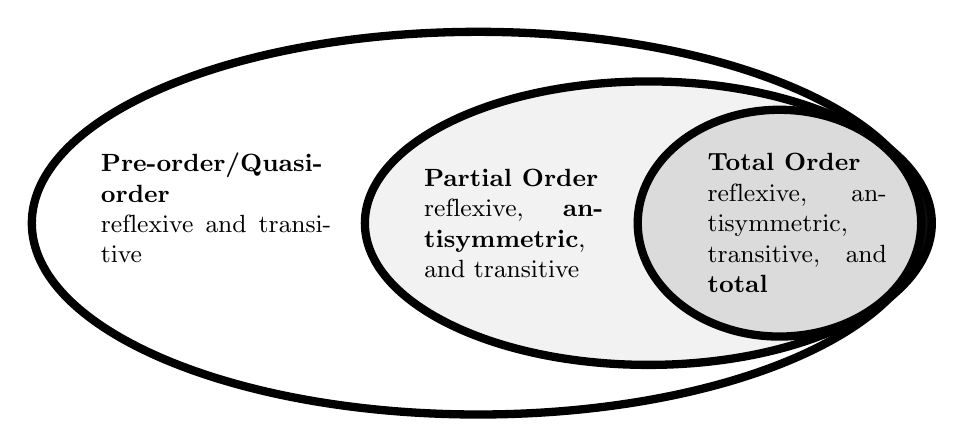
\begin{tikzpicture}[font=\rmfamily\small,scale=.9]
	\drawell{-1}{6.3}{2.7}{0};
	%标记节点,添加文字
	%使用垂直盒子,规定盒子宽度与对齐方式
	\node at (-4.7,0) {\parbox[c]{9em}{\textbf{Pre-order/Quasi-order}\\
			ref\mbox{l}exive and transitive\\}};
	%前两个参数之和为8,才能保证三个椭圆相切于右端点
	\drawell{1.4}{4}{2}{.1};
	\node at (-0.5,0) {\parbox[c]{7em}{\textbf{Partial Order}\\
			ref\mbox{l}exive, \textbf{antisymmetric}, and transitive}};
	
	\drawell{3.25}{2}{1.6}{.2};
	\node at (3.5,0) {\parbox[c]{7em}{\textbf{Total Order}\\
			ref\mbox{l}exive, antisymmetric, transitive, and \textbf{total}}};
	\end{tikzpicture}
	}
}
\end{frame}
\begin{frame}
    \frametitle{Concept Checking List}
    Be familiar with the following:
    \begin{itemize}
        \item covers/adjacent
        \item minimal/minimum element
        \item maximal/maximum element
        \item (in)comparability graph
        \item chain/antichain
        \item lattice: join and meet
    \end{itemize}
    \vv
    \red{\large{Let's see one example!}}
\end{frame}
\begin{frame}
    \frametitle{Example}
    \fbox{
	\parbox{0.95\textwidth}{
	 	\hh Hasse/Order Diagram: edges are the cover pairs $(x, y)$ with $x$ covered by $y$.
	 	\par \phantom{ji}\\
	 	\centering
	 	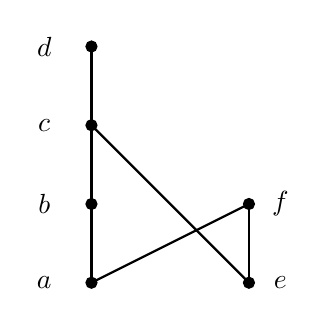
\begin{tikzpicture}
	 	%% vertices
	 	\draw[fill=black] (9,0) circle (2pt);
	 	\draw[fill=black] (9,1) circle (2pt);
	 	\draw[fill=black] (7,0) circle (2pt);
	 	\draw[fill=black] (7,1) circle (2pt);
	 	\draw[fill=black] (7,2) circle (2pt);
	 	\draw[fill=black] (7,3) circle (2pt);
	 	%% vertex labels
	 	\node at (6.4,0) {$a$};
	 	\node at (6.4,1) {$b$};
	 	\node at (6.4,2) {$c$};
	 	\node at (6.4,3) {$d$};
	 	\node at (9.4,0) {$e$};
	 	\node at (9.4,1) {$f$};
	 	%%% edges
	 	\draw[thick] (9,0) -- (9,1);
	 	\draw[thick] (7,0) -- (7,1) -- (7,2) -- (7,3);
	 	\draw[thick] (9,0) -- (7,2);
	 	\draw[thick] (7,0) -- (9,1);
	 	\end{tikzpicture}
	}
}
    \begin{block}{Question}
        \hh Fill in CCP03: ex2-ex6. Do be careful!
    \end{block}
\end{frame}
\begin{frame}
    \frametitle{Exercise}
    1. In the poset $(\mathbb{Z}^+, \mid)$ (where $\mathbb{Z}^+$ is the set of 
    all positive integers and $\mid$ is the divides relation), are the integers 3 and 9 comparable? 
    Are 7 and 10 comparable? \\
    \vs{2em}
    \pause
    \yellow{Solution:}\\
    \hh 3 and 9 are comparable since $3 \mid 9$, \textit{i.e.}, 
    3 divides 9. But 7 and 10 are not comparable since $7 \nmid 10$  
    and $10 \nmid 7$. 
\end{frame}
\begin{frame}
    \frametitle{Exercise}
    2.  A relation $R$ is defined on ordered pairs of integers as follows: $(x,y) R(u,v)$ if $x < u$ and $y > v$. Then $R$ is:
    \begin{enumerate}[(A)]
        \item Neither a partial order nor an equivalence relation
        \item A partial order but not a total order
        \item A total order
        \item An equivalence relation
    \end{enumerate}
    \vs{2em}
    \yellow{Answer:} A
\end{frame}
\begin{frame}
    \frametitle{Exercise}
    3. Given a set $S=\{a, b, c, d\} .$ Consider the following 4 partitions 
    $\pi_{1}, \pi_{2}, \pi_{3}, \pi_{4}$ on $S$: 
    \begin{center}
        $\pi_{1}=\{\overline{a b c d}\}, \pi_{2}=\{\overline{a b}, \overline{c d}\}, \pi_{3}=\{\overline{a b c}, \bar{d}\}, \pi_{4}=\{\bar{a}, \bar{b}, \bar{c}, \bar{d}\} .$ \\
    \end{center}
    \hh Let $p$ be a \textbf{strict} partial order on the set of partitions $S^{\prime}=\left\{\pi_{1}, \pi_{2}, \pi_{3}, \pi_{4}\right\}$ defined as follows: 
    \begin{center}
        $\pi_{i} p \pi_{j}$ if and only if $\pi_{i}$ refines $\pi_{j}$\\ 
    \end{center}
    \hh Find the poset diagram for $\left(S^{\prime}, p\right)$. 
\end{frame}
\begin{frame}
    \frametitle{Solution}
    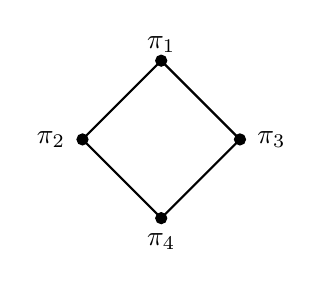
\begin{tikzpicture}
        % vertices
        \draw[fill=black] (0,1) circle (2pt);
        \draw[fill=black] (1,0) circle (2pt);
        \draw[fill=black] (1,2) circle (2pt);
        \draw[fill=black] (2,1) circle (2pt);
        % vertex labels
        \node at (-0.4,1) {$\pi_{2}$};
        \node at (1,-0.3) {$\pi_{4}$};
        \node at (1,2.2) {$\pi_{1}$};
        \node at (2.4,1) {$\pi_{3}$};
        % edges
        \draw[thick] (0,1) -- (1,0) -- (2,1) -- (1,2) -- (0,1);
        \end{tikzpicture}
        \\\hh A partition is said to refine another partition if it splits the sets 
        in the second partition to a larger number of sets.
        \\\hh Therefore, the partial order contains the following ordered pairs: 
        $$\{(\pi_4,\pi_1),(\pi_4,\pi_2),(\pi_4,\pi_3),(\pi_3,\pi_1),(\pi_2,\pi_1)\}$$        
\end{frame}
\section{Cardinality}
\begin{frame}
    \frametitle{Definition}
    \fbox{
	\parbox{0.95\textwidth}{
		\par For any set $A$, we will define a set card $A$ such that
		\begin{itemize}
			\item[-] For any sets $A$ and $B$, $\operatorname{card} A = \operatorname{card} B \Leftrightarrow A \approx B.$
			\item[-] For a finite set $A$, card $A$ is the natural number for which $A \approx n$.
		\end{itemize}
	}
    }
    \\\vv 
    \fbox{
	\parbox{0.95\textwidth}{
		\par Cantor-Schröder-Bernstein Theorem: $$(A \preceq B) \wedge(B \preceq A) \Rightarrow A \approx B.$$
		\par A injection $f$: $A \to B$ and another injection $g$: $B \to A$ $\Rightarrow A \approx B.$ 
	}
    }
    \begin{block}{Why?}
        \hh $\{X \mid \operatorname{card} X =\kappa \}$ is not a set, except for $\kappa = 0$.
    \end{block}
\end{frame}
\begin{frame}
    \frametitle{Explanation for Slides}
    \fbox{
    \parbox{0.95\textwidth}{
		\par Iterate to get a bijection $h : A \to B$:
		$$
		h(x) = \begin{cases}f\,(x), & x \in \bigcup_{k \in \mathbb{N}}(g \circ f\,)^{k}(A-g(B)) \\ g^{-1}(x), & \text { otherwise }\end{cases}
		$$
		\begin{figure}[H]
			\centering
			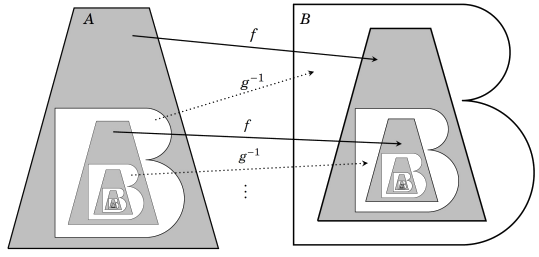
\includegraphics[width=0.7\linewidth]{Iterate}
            %\caption{}
			\label{fig:iterate}
		\end{figure}
	}
}
\end{frame}
\begin{frame}
    \frametitle{Exercise}
    4. Prove the following equinumerosity:
    \begin{itemize}
        \item $\bZ\es\bN$
        \item $\bN \times \bN \es \bN$
        \item $(0,1) \es \bR$
        \item $[0,1] \es (0,1)$
        \item $\calP (\bN) \es \bR$
        \item $\bN^\bN \es \bR$
    \end{itemize}
    \vs{2em}
    \red{Pay attention to the way that you
    build the bijection!}
\end{frame}
\begin{frame}
    \frametitle{Proof: $\bN^\bN \es \bR$}
    \hh We have $2^{\aleph_0} \leq 3^{\aleph_0} \leq 4^{\aleph_0} \leq \dots \leq \aleph_0^{\aleph_0}$, because of the inclusions $\{0, 1\}^\bN \subset \{0,1,2\}^\bN \subset \dots \subset \bN^\bN$. 
    So if we prove that $\aleph_0^{\aleph_0} \leq 2^{\aleph_0}$, then we see that all of these cardinalities are in fact equal. 
    \\\vs{0.5em}
    \hh To show this, we need to find some injection $f: \bN^{\bN} \to \{0, 1\}^\bN$. There are many ways to do this; my favorite is as follows. Let $a = (a_n)$ be some sequence of natural numbers. 
    Then we define $f(a)$ to be the sequence consisting of first $a_0$ ones, followed by a zero, then $a_1$ ones, followed by a zero, then $a_2$ ones, followed by a zero, and so on. 
    This gives a sequence of zeroes and ones, and if $b = (b_n)$ is another sequence of natural numbers, then $f(a) = f(b)$ if and only if $a_n =b_n$ for all indices $n$ if and only if $a = b$. So $f$ is indeed injective, 
    and therefore $\aleph_0^{\aleph_0} \leq 2^{\aleph_0}$.
    \\\vs{0.5em}
    \hh So indeed $2^{\aleph_0} = 3^{\aleph_0} = \dots = \aleph_0^{\aleph_0}$. 
\end{frame}
\begin{frame}
    \frametitle{Thinking}
    A strange thought, why the previous one is wrong?
    \begin{itemize}
        \item Consider $\bN^2,\bN^3,\dots$ is all countable, so $\bN^\bN$ is also countable.
        \item Consider $2^\bN,3^\bN,\dots$ is all equinumerous to $\bR$, so $\bN^\bN$is also equinumerous to $\bR$.
    \end{itemize}
    \vv
    What does this mean?\\
    $$\text{card } \bN = \al ~~~~~\text{card }\bR = \all ~~~~~ \text{card } \bR^\bR = \aleph_2$$

\end{frame}
\section{Leftovers}
\begin{frame}
    \frametitle{Finite Set}
    Important results:
    \begin{itemize}
        \item Let $A$ be any finite set. 
        $f : A \to A$, $f$  injective $\LRarrow$ f
        surjective.
        \item No finite set is equinumerous to a proper subset of itself.
    \end{itemize}
    \vv
    \red{Try to understand them! This may appear in the exam!}
\end{frame}
\begin{frame}
    \frametitle{Longest Increasing Subsequence}
    5. Find the longest increasing/decreasing sequence.
    $$\text{nums }= [10, 9, 2, 5, 3, 7, 101, 18]$$
    \begin{block}{Methodology}
        \begin{table}[]
            \begin{tabular}{||c|ccccccc||}
            \toprule
            num.&0  &1  &2  &3  &4  &5  &6  \\ 
            \midrule
            val.&10  &9  &2  &5  &7  &101  &18  \\ \hline
            len.&1  &1  &1  &2  &3  &4  &4  \\ \hline
            pre.&-  &-  &-  &2  &3  &4  &4  \\ 
            \bottomrule
            \end{tabular}
            \end{table}
    \end{block}
\end{frame}
\section{*Extra Topic}
\begin{frame}
    \frametitle{Prime spiral}
    \begin{figure}[htbp]
        \centering
        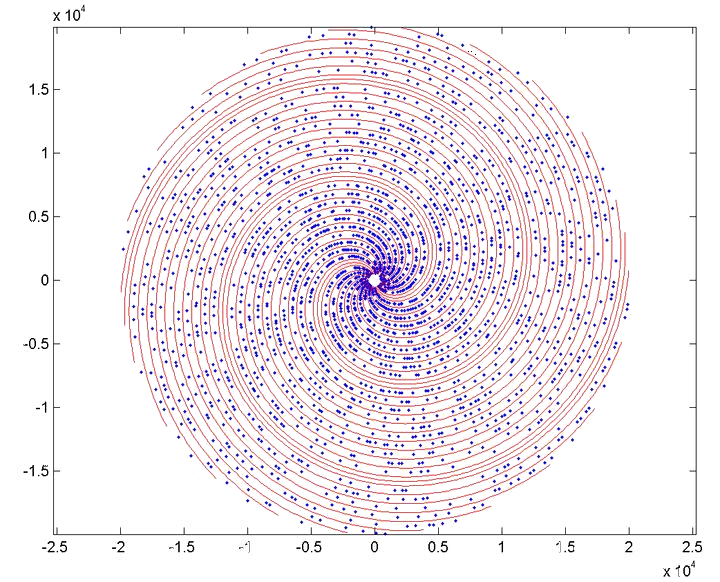
\includegraphics[width=0.55\textwidth]{spiral.png}
    \end{figure}
    Links:
    \begin{itemize}
        \item Zhihu: \url{https://www.zhihu.com/question/24236455}
        \item Bilibili: \url{https://www.bilibili.com/video/BV1tE411h7x4}
    \end{itemize}
\end{frame}
\begin{frame}
    \frametitle{Reference}
    \begin{itemize}
        \item Examples from Dr. Cai Runze's Sildes.
        \item Exercises/graphics from 2021-Fall-Ve203 TA Zhao Jiayuan
        \item What-is-the-result-of-a-number-greater-than-2-raised-to-the-power-of-aleph-0 
        \url{https://math.stackexchange.com/questions/1646830}
    \end{itemize}
\end{frame}
\end{document}